\chapter{自由飞行段弹道特性分析}
\thispagestyle{empty}
\section{自由飞行段弹道方程}
\subsection{自由飞行段假设}
火箭经过动力飞行段在关机点具有一定的位置和速度后,转入无动力、无控制的自由飞行状态。通常作如下假设:

 (1) 载荷在自由段处于真空飞行状态,不受空气动力作用、不必考虑姿态,将火箭看成\red[质点];

 (2) 认为载荷只受\red[]均质圆球]的引力作用,不考虑其他星体的引力影响。

\subsection{轨道方程}
圆形均值地球段引力为
\begin{equation}
	\bm{F}_T = - \dfrac{\mu m}{r^3}\bm{r} = m \dfrac{\d^2 \bm{r}}{\d t^2} \quad \Rightarrow \quad \dfrac{\d^2 \bm{r}}{\d t^2} = - \dfrac{\mu}{r^3} \bm{r}
	\label{4.1}
\end{equation}
引力始终指向$\bm{r}$反方向,$\bm{r}$是由地球中心$O_s$至载荷质心的矢径,所以引力$\bm{F}_T$为一个\dy[有心矢量场]{YXSLC}。

用$\bm{v}$点乘公式\eqref{4.1},可以得到
\begin{equation*}
	\bm{v} \cdot \dfrac{\d \bm{v}}{\d t} = - \dfrac{\mu}{r^3}(\bm{v} \cdot \bm{r}) \quad \Rightarrow \quad \dfrac{1}{2} \dfrac{\d \bm{v}^2}{\d t} = - \dfrac{\mu}{r^3}\left(\dfrac{1}{2}\dfrac{\d \bm{r}^2}{\d t}\right) \quad \Rightarrow \quad \dfrac{1}{2} \dfrac{\d v^2}{\d t} = -\dfrac{\mu}{r^2}\dfrac{\d r}{\d t} = \dfrac{\d }{\d t} \left(\dfrac{\mu}{r}\right)
\end{equation*}
积分后得

\theorem[机械能守恒定律]
{
	\vspace*{-2em}
	\begin{equation}
		\dfrac{1}{2}v^2 = \dfrac{\mu}{r} + E \quad \Rightarrow \quad E = \dfrac{1}{2}v^2 - \dfrac{\mu}{r}
		\label{E}
	\end{equation}
}

进一步,用地心矢叉乘动力学方程\eqref{4.1},有
\begin{equation*}
	\dfrac{\d \bm{r}^2}{\d t^2} = - \dfrac{\mu}{r^3}\bm{r} \quad \Rightarrow \quad \bm{r} \times \dfrac{\d^2 \bm{r}}{\d t^2} = - \dfrac{\mu}{r^3} \bm{r} \times \bm{r} = 0 \quad \Rightarrow \quad \dfrac{\d }{\d t}\left(\bm{r} \times \dfrac{\d \bm{r}}{\d t}\right) = \dfrac{\d }{\d t}(\bm{r} \times \bm{v}) = 0
\end{equation*}
即得到

\theorem[动量矩守恒]
{
	\vspace*{-2em}
	\begin{equation}
		\bm{r} \times \bm{v} = \bm{h}
	\end{equation}
}
\noindent 由于火箭动量矩守恒,因此自由段运动为平面运动,由关机点参数$\bm{r}_k,\bm{v}_k$决定。

动力学方程两边叉乘动量矩,则有\\
左式
\begin{equation*}
	\dfrac{\d^2 \bm{r}}{\d t^2} \times \bm{h} = \dfrac{\d }{\d t}\left(\dfrac{\d \bm{r}}{\d t} \times \bm{h}\right)
\end{equation*}
右式
\begin{align*}
	- \dfrac{\mu}{r^3} \bm{r} \times \bm{h} &= - \dfrac{\mu}{r^3}\bm{r} \times (\bm{r} \times \bm{v})\\
	& = -\dfrac{\mu}{r^3} \big[\bm{r} \cdot (\bm{r} \cdot \bm{v}) - \bm{v} \cdot (\bm{r} \cdot \bm{r})\big] \\
	& = - \dfrac{\mu}{r^3}\big[r \dot{r} \bm{r} - r^2 \bm{v}\big]\\
	& = - \mu \left[\dfrac{\bm{r}}{r^2}\dfrac{\d r}{\d t} - \dfrac{1}{r} \dfrac{\d \bm{r}}{\d t}\right]\\
	& = \mu \dfrac{\d}{\d t}\left(\dfrac{\bm{r}}{r}\right)
\end{align*}
即
\begin{equation}
	\dfrac{\d }{\d t}\left(\dfrac{\d \bm{r}}{\d t} \times \bm{h}\right) = \mu \dfrac{\d }{\d t}\left(\dfrac{\bm{r}}{r}\right)
\end{equation}
积分可得
\begin{equation}
	\dfrac{\d \bm{r}}{\d t} \times \bm{h} = \mu \left(\dfrac{\bm{r}}{r} + \bm{e}\right)
\end{equation}

为了获得标量方程,可以点乘$\bm{r}$,有
\begin{equation*}
	\begin{cases}
		\, \mu \bm{r} \cdot \left(\dfrac{\bm{r}}{r} + \bm{e}\right) = \mu \big[r + re\cos <\bm{r}, \bm{e}>\big]\\[1em]
		\, \bm{r}\cdot\left(\dfrac{\d \bm{r}}{\d t} \times \bm{h}\right) = \bm{h} \cdot \left(\bm{r} \times \dfrac{\d \bm{r}}{\d t}\right) = h^2 
	\end{cases}
\end{equation*}
即

\theorem[自由飞行段的轨道方程式]
{
	\vspace*{-2em}
	\begin{align}
		\dfrac{\d \bm{r}}{\d t} \times \bm{h} &= \mu \left(\dfrac{\bm{r}}{r} + \bm{e}\right)\\
		r = \dfrac{h^2 / \mu}{1 + e \cos <\bm{r}, \bm{e}>} &\triangleq \dfrac{P}{1 + e \cos <\bm{r}, \bm{e}>}
	\end{align}
}

\section{弹道方程的分析}
\subsection{符号$e,P$的意义及其确定}
轨道方程式对应为圆锥截线方程式,$e$为偏心率,决定圆锥截线形状,$P$为半通径,和$e$共同决定截线尺寸。建立关机点当地坐标系$\bm{K-ijk}$,显然$\bm{k}$与动量矩$\bm{h}$方向一致。
\begin{equation}
	\dfrac{\bm{r}}{\d t} \times \bm{h} = \mu \left(\dfrac{\bm{r}}{r} + \bm{e}\right) \quad \Rightarrow \quad \bm{v} \times \dfrac{\bm{h}}{\mu} = \dfrac{\bm{r}}{r} + \bm{e}
\end{equation}
其中,
\begin{equation}
	h = \left|\bm{r} \times \bm{v}\right| = rv \cos \varTheta
	\label{h}
\end{equation}
其中$\varTheta$为\dy[当地速度倾角]{DDSDQJ},则
\begin{equation}
	\bm{v} \times \dfrac{\bm{h}}{\mu} = 
	\begin{vmatrix}
		\bm{i} & \bm{j} & \bm{k}\\
		v_k\sin \varTheta & v_k \cos \varTheta & 0 \\
		0 & 0 & r_kv_k\cos \varTheta/\mu
	\end{vmatrix}
	= 
	\begin{bmatrix}
		r_kv_k^2 \cos^2 \varTheta / \mu \\
		-r_kv_k^2 \sin \varTheta \cos \varTheta / \mu \\
		0
	\end{bmatrix}
\end{equation}
定义\dy[能量参数]{NLCS}(表示动能与势能之比)为
\begin{equation}
	\nu_k = \dfrac{v_k^2}{\mu / r_k}
\end{equation}
进一步,可以计算得到
\begin{equation}
	\bm{e} = \bm{v} \times \dfrac{\bm{h}}{\mu} - \dfrac{\bm{r}}{r} = 
	\begin{bmatrix}
		\nu \cos^2 \varTheta - 1\\
		-\nu \cos \varTheta \cos \varTheta\\
		0
	\end{bmatrix}
\end{equation}
则

\theorem[$e,P$的计算值]
{
	\vspace*{-2em}
	\begin{align}
		e &= \sqrt{1 + \nu_k(\nu_k - 2)\cos^2 \varTheta_k} \label{e}\\[0.5em]
		P = \dfrac{h^2}{\mu} &= \dfrac{r_k^2 v_k^2 \cos^2 \varTheta_k}{\mu} = r_k v_k \cos^2 \varTheta_k \label{P}
	\end{align}
	在$e,P$已知的情况下,轨道上任意一点的地心矢径大小$r$仅与夹角$<\bm{r},\bm{e}>$有关,记
	\begin{itemize}
		\item $f = <\bm{r}, \bm{e}>$ \quad 定义由$\bm{e}$矢量顺飞行方向到r矢量为正角,称为\dy[真近点角]{ZJDJ}
		\item $\cos f = \dfrac{P - r}{re}$ \quad 由关机点$\bm{r}_k$矢量反向转$f$角即可确定$\bm{e}$矢量方向
	\end{itemize}
	当$f = 0$时,轨道地心矢径$\bm{r}_p$最小,称点$p$为近地点,因此$\bm{e}$矢量与$\bm{r}_p$矢径方向一致。
}

则各个物理量可以表示为

\sssection[地心距(轨道方程)]
\begin{equation}
	r = \dfrac{P}{1 + e \cos f}
\end{equation}

\sssection[径向速度]
\begin{equation}
	\begin{cases}
		\, v_r = \dot{r} = \dfrac{P}{\left(1 + e \cos f\right)^2} e \sin f \cdot \dot{f} \\[0.8em]
		\, \dot{f} = \dfrac{h}{r^2} = \dfrac{1}{r} \sqrt{\dfrac{\mu}{P}}(1 + e \cos f)
	\end{cases}
	\quad \Rightarrow \quad v_r = \sqrt{\dfrac{\mu}{P}}e \sin f
\end{equation}

\sssection[周向速度]
\begin{equation}
	v_f = r\dot{f} = \sqrt{\dfrac{\mu}{P}}(1 + e \cos f)
\end{equation}

\sssection[速度及其倾角]
\begin{align}
	v = \sqrt{\dfrac{\mu}{P} \left(1 + 2 e \cos f + e^2\right)} \\
	\tan \varTheta = \dfrac{v_r}{v_f} = \dfrac{e \sin f}{1 + e \cos f}
\end{align}

\subsection{轨道根数}
对于导弹而言,关机点参数用于确定被动段参数,从而获取落点参数。但对于运载火箭,其有效载荷为入轨的人造卫星,因此需要给出其轨道根数。

\defination[轨道根数]
{
	\vspace*{-2em}
	{
		\begin{enumerate}[\hspace*{2em}]
			\item \dy[升交点]{SJD} \quad 卫星从南向北穿越赤道点\vspace*{-0.5em}
			\item \dy[春分点]{CFD} \quad 2000年1月1.5日的平春分点\vspace*{-0.5em}
			\item \dy[长半轴$a$]{CBZ} \quad 圆锥截线轨道大小参数\vspace*{-0.5em}
			\item \dy[偏心率$e$]{PXL} \quad 圆锥截线轨道形状参数\vspace*{-0.5em}
			\item \dy[轨道倾角$i$]{GDQJ} \quad 轨道面与赤道面的夹角\vspace*{-0.5em}
			\item \dy[近地点角距$w$]{JDDJJ} \quad 升交点与近地点夹角\vspace*{-0.5em}
			\item \dy[升交点角距$\Omega$]{SJDJJ} \quad 升交点与春分点夹角\vspace*{-0.5em}
			\item \dy[近地点时刻$t_p$]{JDDSK} \quad 飞越近地点的时刻
		\end{enumerate}
	
	}
}

\subsection{轨道形状与关机点参数}
轨道所对应的圆锥截线形状由偏心率$e$决定。由\peref[E]和\peref[h],注意到有
\begin{equation}
	E = \dfrac{1}{2} v_k^2 - \dfrac{\mu}{r_k}  \quad \Rightarrow \quad \nu_k = \dfrac{r_k v_k^2}{\mu} = 2\left(1 + \dfrac{r_kE}{\mu}\right), \quad \cos^2 \varTheta_k = \dfrac{h^2}{r_k^2 v_k^2}
\end{equation}
则偏心率可改写为
\begin{equation}
	e = \sqrt{1 + \nu_k (\nu_k - 2)\cos^2 \varTheta_k} = \sqrt{1 + 2 \dfrac{h^2}{\mu^2}E} = \sqrt{1 + 2 \dfrac{P}{\mu} E}
\end{equation}

\sssection[$e = 0$时轨道为圆]

\noindent 轨道参数如下:

(1) 地心距
\begin{equation}
	r = \dfrac{P}{1 + e \cos f} = P = r_k
\end{equation}

(2) 速度倾角
\begin{equation}
	\varTheta = \varTheta_k = 0
\end{equation}

(3) 偏心率
\begin{equation}
	e =  \sqrt{1 + \nu_k (\nu_k - 2)\cos^2 \varTheta_k} = 0
\end{equation}

(4) 能量参数
\begin{equation}
	\nu = \nu_k = 1
\end{equation}

(5) 速度
\begin{equation}
	v = v_k = \sqrt{\dfrac{\mu}{r_k}} \triangleq v_{\text{\RMN[1]}}\, \mbox{(\dy[第一宇宙速度]{DYYZSD})}
\end{equation}

\sssection[$e = 1$时轨道为抛物线]

\noindent 轨道参数如下:

(1) 能量参数
\begin{equation}
	e =  \sqrt{1 + \nu_k (\nu_k - 2)\cos^2 \varTheta_k} = 1 \quad \Rightarrow \quad \nu_k = 2
\end{equation}

(2) 能量
\begin{equation}
	e = \sqrt{1 + 2 \dfrac{P}{\mu}E} = 1 \quad \Rightarrow \quad E = 0
\end{equation}

(3) 速度
\begin{equation}
	v = v_k = \sqrt{2\dfrac{\mu}{r_k}} \triangleq v_{\text{\RMN[2]}}\, \mbox{(\dy[第二宇宙速度]{DEYZSD})}
\end{equation}

\sssection[$e > 1$时轨道为双曲线]

\noindent 轨道参数如下:

(1) 能量参数
\begin{equation}
	e =  \sqrt{1 + \nu_k (\nu_k - 2)\cos^2 \varTheta_k} > 1 \quad \Rightarrow \quad \nu_k > 2
\end{equation}

(2) 双曲线\dy[剩余速度]{SYSD}
\begin{equation}
	E>0 \quad \Rightarrow \quad \dfrac{v_k^2}{2} - \dfrac{\mu}{r_k} = \dfrac{v_\infty^2}{2}
\end{equation}

\sssection[$e < 1$时轨道为椭圆]

\noindent 轨道参数如下:

(1) 能量参数
\begin{equation}
	e =  \sqrt{1 + \nu_k (\nu_k - 2)\cos^2 \varTheta_k} \in (0,1) \quad \Rightarrow \quad 1 < \nu_k < 2
\end{equation}

(2) 速度
\begin{equation}
	E<0 \quad \Rightarrow \quad v_k < v_{\text{\RMN[2]}}
\end{equation}
质点动能不足以将质点移动到无穷远处,地心矢径有限。
\vspace*{0.5em}

\sssection[总结]

(1) \dy[弹道]{DD} \quad 运载火箭及其载荷的飞行轨迹,不闭合。

(2) \dy[轨道]{GD}\quad 人造卫星等绕地球闭合飞行轨迹活动。

(3) \dy[星际航行]{XJHX}\quad 能量参数$\nu_k \ge 2$。

(4) \dy[绕地飞行]{RDFX} \quad 能量参数$\nu_k < 2$:
$
\begin{cases}
	\, \mbox{圆形轨道}\quad \varTheta_k = 0 \quad v_k = v_{\text{\RMN[1]}}\\
	\, \mbox{椭圆轨道}\quad 
	\begin{cases}
		\, \mbox{闭合轨道} \\
		\, \mbox{不闭合轨道}
	\end{cases}
\end{cases}
$

\sssection[椭圆轨道的进一步分析]

椭圆直角坐标方程为
\begin{equation}
	\dfrac{x^2}{a^2} + \dfrac{y_2}{b^2} = 1, \quad c= \sqrt{a^2 + b^2}
\end{equation}
其中,$a,b,c$分别为椭圆的长半轴、短半轴、半焦距。根据轨道方程的近地点和远地点,可得
\begin{equation}
	\begin{cases}
		\, f = 0 \quad r_p = r_{\min} = \dfrac{P}{1 + e} \\
		\, f = \pi \quad r_a = r_{\max} = \dfrac{P}{1 - e}
	\end{cases}
\end{equation}
可以求得椭圆轨道的参数
\begin{align}
	a &= \dfrac{r_a + r_p}{2} = \dfrac{P}{1 - e^2}\\[0.5em]
	c &= \dfrac{r_a - r_p}{2} = \dfrac{eP}{1 - e^2} = ea \\[0.5em]
	b &= \sqrt{a^2 - c^2} = \dfrac{P}{\sqrt{1 - e^2}}\\[0.5em]
	e &= \dfrac{a}{c} = \sqrt{1 - \left(\dfrac{b}{a}\right)^2}\\[0.5em]
	P &= \dfrac{b^2}{a}
\end{align}
且
\begin{equation}
	e = \sqrt{1 + 2 \dfrac{P}{\mu}E} = \sqrt{1 - \left(\dfrac{b}{a}\right)^2},\quad P = \dfrac{b^2}{a} \quad \Rightarrow \quad a = -\dfrac{\mu}{2E} = - \dfrac{\mu r_k}{r_kv_k^2 - 2\mu}
\end{equation}
则

\theorem[活力公式]
{
	椭圆的长半轴只与主动段关机点的机械能$E$有关,且$E<0$。$E$越大,$a$也越大,同时有
	\begin{equation}
		v^2 = \mu \left(\dfrac{2}{r} - \dfrac{1}{a}\right)
	\end{equation}
}

\sssection[人造卫星条件]

根据轨道形状与关机点参数的关系可知,在基本假设条件下,满足以下条件可使轨道不与地球相交:
\begin{equation}
	\begin{cases}
		\, \mbox{圆形轨道}\quad \varTheta_k = 0 , \nu_k = 1\\
		\, \mbox{椭圆轨道}\quad 1 < \nu_k < 2, r_{\min} > R_{\text{e}}
	\end{cases}
\end{equation}
但考虑到地球外的大气层,即使100km处大气密度十分稀薄,但卫星速度很高,大气会显著地阻碍卫星运动,使其速度降低,从而使轨道近地点高度下降,最终卫星失去功能。因此必须使卫星运行在离地面的一定高度上,称此高度为\dy[生存高度]{SCGD},记为$h_L$,该高度与卫星轨道停留时间相关。所以有
\begin{equation}
	r_p \ge r_L = R_{\text{e}} + h_L
\end{equation}
那么,各个参数满足以下关系:

(1) 地心距
\begin{equation*}
	r_k \ge r_p \ge r_L
\end{equation*}

(2) 速度倾角(由\peref[e]及\peref[P])
\begin{equation*}
	r_p = \dfrac{P}{1 + e} \ge r_L \quad \Rightarrow \quad \cos \varTheta_k \ge \dfrac{r_L}{r_k} \sqrt{1 + \dfrac{2 \mu}{v_k^2}\left(\dfrac{1}{r_L} - \dfrac{1}{r_k}\right)} \quad \Rightarrow \quad \cos \varTheta_k \ge \dfrac{r_L}{r_k} \sqrt{1 + \dfrac{2}{\nu_k}\left(\dfrac{r_k}{r_L} - 1\right)} 
\end{equation*}

(3) 速度
\begin{equation*}
	\dfrac{r_L}{r_k} \sqrt{1 + \dfrac{2 \mu}{v_k^2}\left(\dfrac{1}{r_L} - \dfrac{1}{r_k}\right)} \le \cos \varTheta_k \le 1 \quad \Rightarrow \quad v_k^2 \ge \dfrac{2 \mu r_L}{r_k(r_k + r_L)}  \quad \Rightarrow \quad \nu_k \ge \dfrac{2}{1 + r_k/r_L}
\end{equation*}


因此只有关机点参数满足上述(1)和(2)或(3)项条件,才能使其载荷称为人造卫星。

\section{射程与主动段终点参数的关系}
\noindent 需要解决的问题:\vspace*{-0.5em}
\begin{itemize}
	\item 已知关机点的状态参数,计算导弹的射程。\vspace*{-0.3em}
	\item 已知导弹的射程,反求导弹的关机条件。
\end{itemize}

\subsection{被动段射程的计算}
\defination[导弹射程]
{
	考虑地球为均质圆球,自由段弹道处于关机点平面内,弹道平面与地球表面的截痕为大圆弧,则有\dy[射程]{SC}
	\begin{align}
		L_{kc} &= L_{ke} + L_{ec} \\
		L_{ke} &= R \beta_e
	\end{align}
	由上式则射程可用相应的地心角描述,称为\dy[角射程]{JSC}。导弹在再入段受到气动力作用,其弹道不是椭圆的一部分,但其射程所占比例很小,可近似看成椭圆弹道的延续,则整个被动段弹道用椭圆来描述。
	\begin{equation}
		L_{kc} \approx R\beta_c \quad \beta_c = \beta_e + \beta_{ec}
	\end{equation}
	若能找到射程角与关机点状态关系即找到了射程与关机点状态的关系。
}
\begin{figure}[!htb]
	\centering
	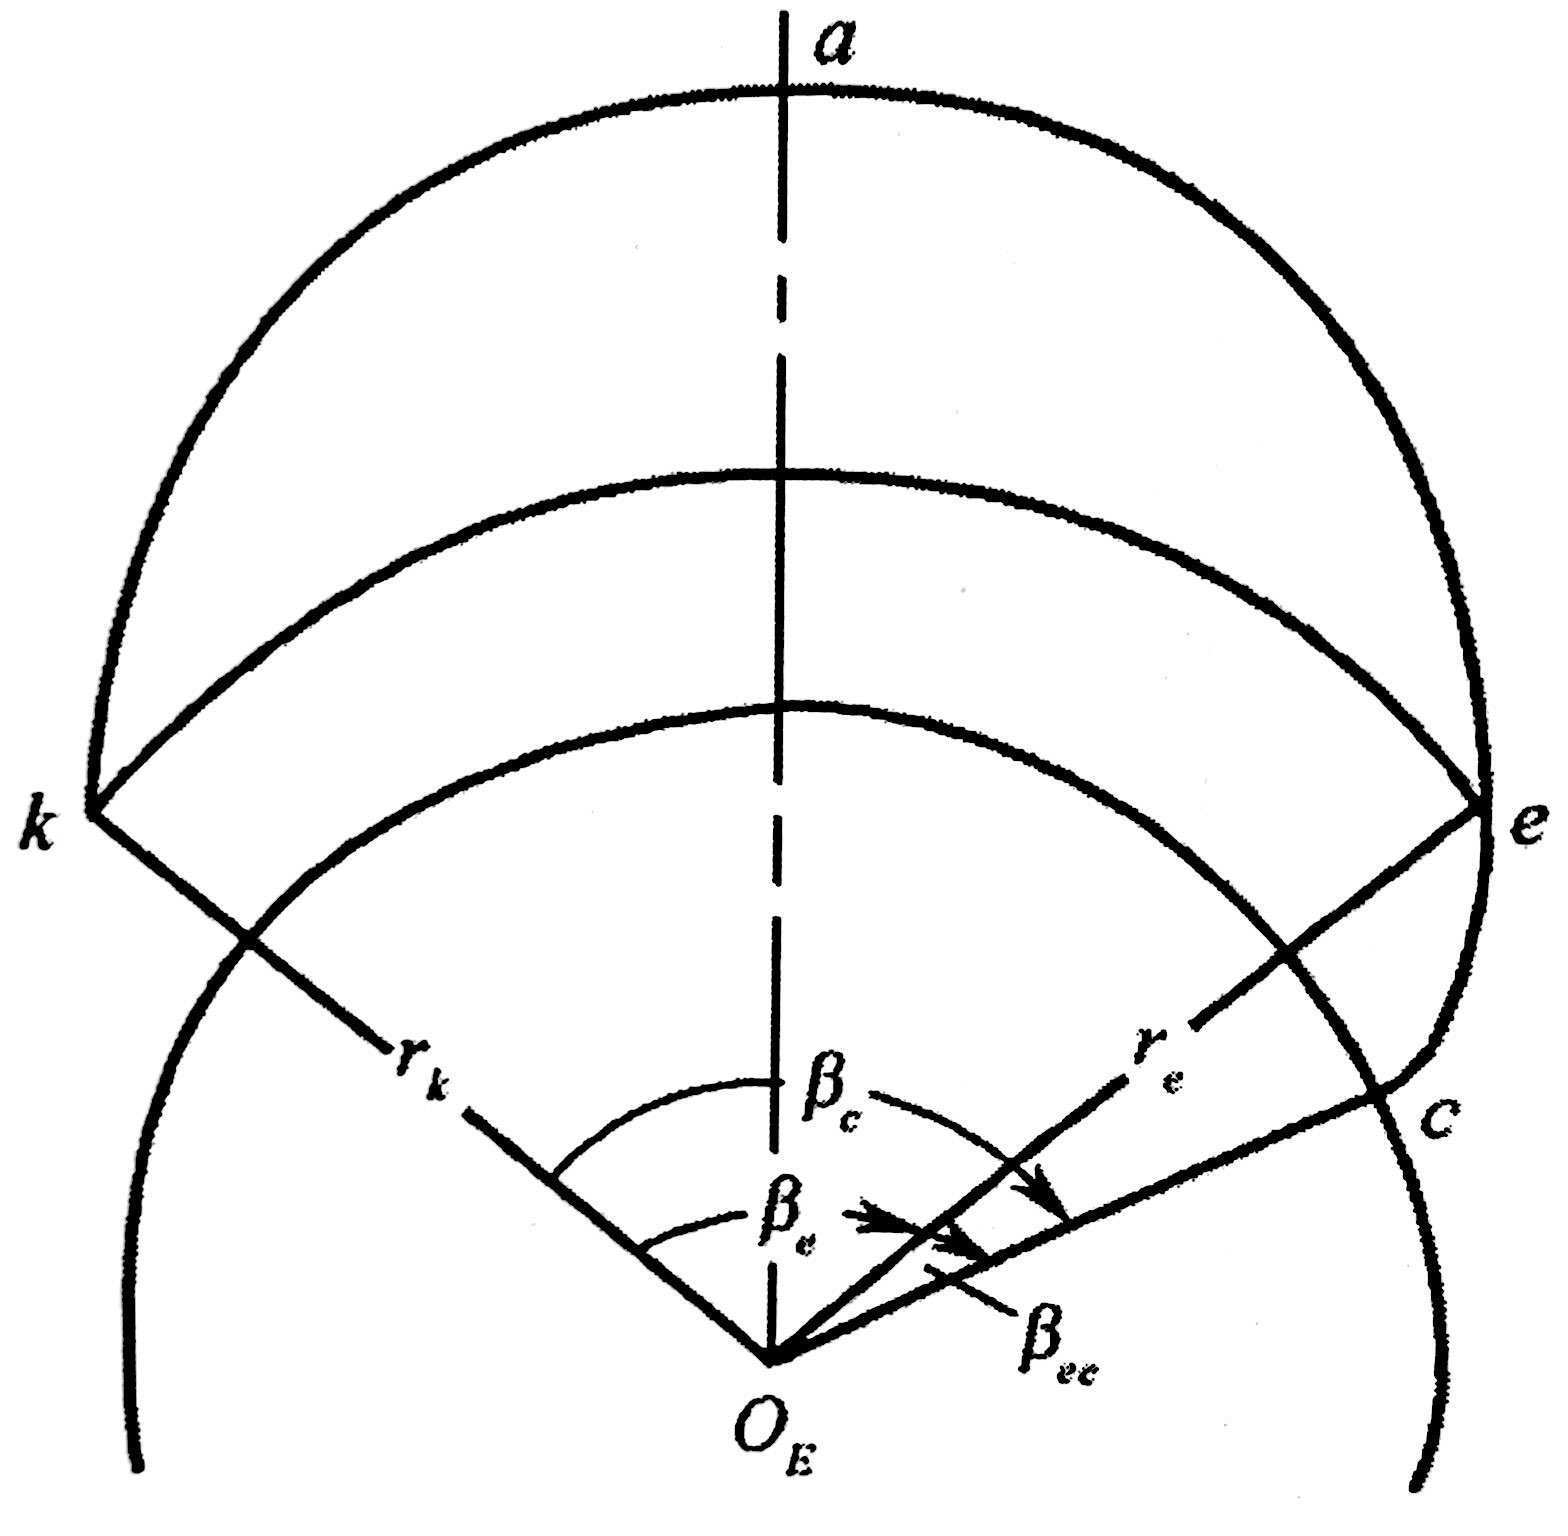
\includegraphics[width=0.3\linewidth]{pic/导弹射程.jpg}
	\caption{自由段、被动段的射程角}
	\label{射程角}
\end{figure}

如图 \ref{射程角} 所示,已知$K,C$是椭圆弹道上的两点,他们的矢径与近地点极轴之间的夹角(真近点角)记为$f_k, f_c$,结合椭圆方程的轨道表达式,可以得到
\begin{equation}
	\beta_c = f_c - f_k,\quad \cos f = \dfrac{P - r}{er}
\end{equation}
当主动段终点参数给定,那么$f$仅仅是$r$的函数,即
\begin{equation}
	\begin{cases}
		\, \cos f_k = \dfrac{P - r_k}{e r_k}\\[0.5em]
		\, \cos f_c = \dfrac{P - r_c}{er_c} \approx \dfrac{P - R}{eR} 
	\end{cases}
\end{equation}
考虑到椭圆弹道的对称性,有:$\angle KO_E a = \angle aO_Ee = \dfrac{\beta_e}{2}$,则
\begin{equation}
	\begin{cases}
		\, \cos f_k = \cos \left(\pi - \dfrac{\beta_e}{2}\right) = \dfrac{P - r_k}{e r_k}\\[0.5em]
		\, \cos f_c = \cos\left(f_k + \beta_c\right) = \cos \left(\pi + \beta_c - \dfrac{\beta_e}{2}\right) = - \cos \left(\beta_c - \dfrac{\beta_e}{2}\right) = \dfrac{P - R}{eR} 
	\end{cases}
\end{equation}
化简,得
\begin{equation*}
	 \cos \dfrac{\beta_e}{2} = \dfrac{r_k - P}{e r_k} \quad \Rightarrow \quad \sin \dfrac{\beta_e}{2} = \dfrac{1}{e} \sqrt{e^2 - \left(1 - \dfrac{P}{r_k}\right)^2}
\end{equation*}
将$e, P$的表达式代入,得
\begin{equation}
	\begin{cases}
		\, e = \sqrt{1 + \nu_k(\nu_k - 2)\cos^2 \varTheta_k} \\[0.5em]
		P = \dfrac{r_k^2 v_k^2\cos ^2 \varTheta_k}{\mu} = r_k\nu_k\cos^2 \varTheta_k
	\end{cases}
	\quad \Rightarrow \quad \sin \dfrac{\beta_e}{2} = \dfrac{1}{e} \sqrt{e^2 - \left(1 - \dfrac{P}{r_k}\right)^2} = \dfrac{P}{er_k}\tan \varTheta_k
	\label{beta_e}
\end{equation}
将$\beta_e$的表达式代入
\begin{equation*}
	\begin{cases}
		\cos \dfrac{\beta_e}{2} = \dfrac{r_k - P}{e r_k}\\[0.5em]
		\sin \dfrac{\beta_e}{2} = \dfrac{P}{er_k}\tan \varTheta_k
	\end{cases}
\quad \xrightarrow{\,\,\,\mbox{\scriptsize 代入}\,\,\,}	\quad \cos \left(\beta_c - \dfrac{\beta_e}{2}\right) = \cos \beta_c \cos \dfrac{\beta_e}{2} + \sin\beta_c \sin \dfrac{\beta_e}{2} = \dfrac{R-P}{eR}
\end{equation*}
可以得到
\begin{equation*}
	\begin{split}
		&\left(1 - \dfrac{P}{r_k}\right)\cos \beta_c + \dfrac{P}{r_k} \tan \varTheta_k\sin \beta_c = 1 - \dfrac{P}{R}\\[0.5em]
		\xrightarrow{\,\, \textstyle P = r_k\nu_k\cos^2 \varTheta_k\,\,}\quad & (1-\nu_k \cos^2 \varTheta_k)\cos \beta_c + \nu_k \cos^2 \varTheta_k\tan \varTheta_k \tan \varTheta_k \sin \beta_c = 1 - \dfrac{r_k \nu_k \cos^2 \varTheta_k}{R}\\[0.5em]
		\Rightarrow \quad & \dfrac{r_k}{R} = \dfrac{1 - (1-\nu_k\cos^2 \varTheta_k) \cos \beta_c + \nu_k \cos^2 \varTheta_k\tan\varTheta_k\sin \beta_c}{\nu_k \cos^2 \varTheta_k}
	\end{split}
\end{equation*}
最终,我们可以得到

\theorem[命中方程]
{
	\vspace*{-1.5em}\index{MZFC@命中方程}
	\begin{equation}
		\dfrac{r_k}{R} = \dfrac{1 - \cos \beta_c}{\nu_k \cos^2 \varTheta_k} + \dfrac{\cos \left(\beta_c + \varTheta_k\right)}{\cos \varTheta_k}
	\end{equation}
	三角函数转换为半角形式有
	\begin{equation*}
		\cos \beta_c = \dfrac{1 - \tan^2 \dfrac{\beta_c}{2}}{1 + \tan^2 \dfrac{\beta_c}{2}}\qquad \sin \beta_c = \dfrac{2 \tan \dfrac{\beta_c}{2}}{1 + \tan^2 \dfrac{\beta_c}{2}}
	\end{equation*}
	代入命中方程,得到
	\begin{equation}
		\big[2R\left(1 + \tan^2\varTheta_k\right) - \nu_k (R + r_k)\big]\tan^2 \dfrac{\beta_c}{2} - 2\nu_k R \tan \varTheta_k \tan \dfrac{\beta_c}{2} + \nu_k \left(R - r_k\right) = 0
		\label{命中方程}
	\end{equation}
	由于轨道参数已知,则方程可以简化为
	\begin{equation}
		A \cdot \tan^2 \dfrac{\beta_c}{2} - B \cdot \tan \dfrac{\beta_c}{2} + C = 0
	\end{equation}
}
其中,
\begin{equation*}
	\begin{split}
		A &= 2r_c \left(1 + \tan^2 \varTheta_k\right) - \nu_k (r_c + r_k) \\
		& \ge 2r_c \left(1 + \tan^2 \varTheta_k\right) -2 \nu_k r_k \\
		& = 2r_c \left(1 + \tan^2 \varTheta_k\right) -2P/\cos^2 \varTheta_k \\
		& = 2r_c \left(1 + \tan^2 \varTheta_k\right) \left(1 - \dfrac{P}{r_c}\right)\\
		& = 2r_c \left(1 + \tan^2 \varTheta_k\right) -\big[1 - (1 + e\cos f_c)\big]\\
		& = -2r_c \left(1 + \tan^2 \varTheta_k\right)e \cos f_c\\
		& \ge 0\\
		C &=  \nu_k (r_c - r_k) \le 0
	\end{split}
\end{equation*}

\theorem[被动段射程计算公式]
{
	射程通常小于$180\degree$,因此被动段射程计算公式为
	\begin{equation}
		\tan \dfrac{\beta_c}{2} = \dfrac{B + \sqrt{B^2 - 4AC}}{2A} , \quad L_{kc} = R \beta_c
		\label{被动段}
	\end{equation}	
	其中,
	\begin{equation}
		\begin{cases}
			\, A = 2 R \big(1 + \tan^2 \varTheta_k\big) - \nu_k \big(R + r_k\big)\\
			\, B = 2 \nu_k R \tan \varTheta_k \\
			\, C = \nu_k \big(R - r_k\big)
		\end{cases}
		\label{被动段系数}
	\end{equation}
}

\subsection{自由段射程的计算}

由被动段段射程公式,只需要把$r_e = r_k$替换掉$R$即可,即

\theorem[自由段射程计算公式]
{
	\vspace*{-2em}
	\begin{equation}
		\tan \dfrac{\beta_e}{2} = \dfrac{B + \sqrt{B^2 - 4AC}}{2A} 
	\end{equation}	
	其中,
	\begin{equation}
		\begin{cases}
			\, A = 2 r_k \big(1 + \tan^2 \varTheta_k\big) - 2\nu_k r_k\\
			\, B = 2 r_k \nu_k  \tan \varTheta_k \\
			\, C = \nu_k \big(r_k - r_k\big) = 0
		\end{cases}
	\label{自由段系数}
	\end{equation}
	简化为
	\begin{equation}
		\tan \dfrac{\beta_c}{2} \approx \tan \dfrac{\beta_e}{2} = \dfrac{B}{A} = \dfrac{\nu_k \sin \varTheta_k \cos \varTheta_k}{1 - \nu_k \cos^2 \varTheta_k}
		\label{自由段方程}
	\end{equation}
	实际上,将\peref[P]$\,\, P = r_k \nu_k \cos^2 \varTheta_k$代入\peref[beta_e],可以得到
	\begin{equation}
		\sin \dfrac{\beta_c}{2} \approx \sin \dfrac{\beta_e}{2} = \dfrac{\nu_k}{2 e}\sin 2 \varTheta_k
		\label{自由段}
	\end{equation}
	工程上常用这个形式进行计算,其比较简单。自由段射程为
	\begin{equation}
		L_{ke} = R \cdot \beta_e
	\end{equation}
}

\clearpage
观察自由段射程公式\eqref{自由段},可以发现

\textbf{(1) \hspace*{0.5em} 能量系数给定}\\
\hspace*{2em} 存在\red[最佳速度倾角使射程最大]。也就是说,在给定关机点矢径及速度下,亦即给定机械能$E$下,最佳速度倾角使射程最大。
\begin{equation*}
	\varTheta_{k\text{.opt}} \quad \Rightarrow \quad \beta_{c\text{.max}}
\end{equation*}

\textbf{(2) \hspace*{0.5em} 射程给定}\\
\hspace*{2em} 存在\red[最佳速度倾角使能量系数最小],当关机点位置定,即使关机点速度最小,也就是说导弹的机械能E最小。称为\dy[最小能量弹道]{ZXNLDD}。


\subsection{最佳倾角确定}

已知$r_k, v_k$,确定$\varTheta_{k\text{.opt}}, \beta_{c\text{.max}}$。

被动段射程可以描述为$\beta_c = \beta_c\big(r_k, v_k, \varTheta_k\big)$,由于$r_k, v_k$确定,则$\beta_c = \beta_c\big(\varTheta_k\big)$,极值点(最佳倾角)处导数为0,即
\begin{equation}
	\dfrac{\partial \beta_c}{\partial \varTheta_k} = 0
\end{equation}

对方程\eqref{自由段方程}求导可得
\begin{equation}
	\dfrac{\partial A}{\partial \varTheta_k} \tan^2 \dfrac{\beta_c}{2} - \dfrac{\partial B}{\partial \varTheta_k} \tan \dfrac{\beta_c}{2} + \left(2 A \tan \dfrac{\beta_c }{2} - B\right)\dfrac{\partial \tan \dfrac{\beta_c}{2}}{\partial \varTheta_k} = 0
\end{equation}
对自由段方程的系数\eqref{被动段系数}求导,可以得到
\begin{equation}
	\begin{cases}
		\, \dfrac{\partial A}{\partial \varTheta_k} = 4R\tan \varTheta_k\sec^2\varTheta_k \\[0.8em]
		\, \dfrac{\partial B}{\partial \varTheta_k} = 2R\nu_k \sec^2 \varTheta_k
	\end{cases}
\end{equation}
且
\begin{equation}
	\dfrac{\partial \tan \dfrac{\beta_c}{2}}{\partial \varTheta_k} = \dfrac{1}{2} \sec^2 \dfrac{\beta_c}{2} \dfrac{\partial \beta_c}{\partial \varTheta_k} = 0(\varTheta_k = \varTheta_{k\text{.opt}}, \beta_c = \beta_{c\text{.max}})
\end{equation}

取$\varTheta_k = \varTheta_{k\text{.opt}}, \beta_c = \beta_{c\text{.max}}$,则
\begin{align*}
	& 4 R \tan \varTheta_{k\text{.opt}} \sec^2\varTheta_{k\text{.opt}} \tan^2 \dfrac{\beta_{c\text{.max}}}{2} - 2 R \nu_k \sec^2 \varTheta_{k\text{.opt}} \tan \dfrac{\beta_{c\text{.max}}}{2} = 0 \\
	\Longrightarrow \quad & 2R\sec^2 \varTheta_{k\text{.opt}} \tan \dfrac{\beta_{c\text{.max}}}{2} \left(2 \tan \varTheta_{k\text{.opt}} \tan \dfrac{\beta_{c\text{.max}}}{2} - \nu_k\right) = 0 \\
	\xrightarrow{ \,\, \textstyle 2R\sec^2 \varTheta_{k\text{.opt}} \tan \frac{\textstyle \beta_{c\text{.max}}}{\textstyle 2} \neq 0 \,\, } \quad & 2 \tan \varTheta_{k\text{.opt}} \tan \dfrac{\beta_{c\text{.max}}}{2} - \nu_k = 0
\end{align*}
即
\begin{equation}
	\tan \dfrac{\beta_{c\text{.max}}}{2} = \dfrac{\nu_k}{2 \tan \varTheta_{k\text{.opt}}}
\end{equation}
将计算结果代入到\peref[命中方程],化简后可以得到
\begin{equation}
	\big[4(R - r_k) - 2 R \nu_k\big] \tan^2 \varTheta_{k\text{.opt}} = \nu_k^2 (R + r_k) - 2 R \nu_k
\end{equation}

\theorem[被动段最佳速度倾角]
{
	\vspace*{-1em}
	\begin{equation}
		\tan \varTheta_{k\text{.opt}} = \sqrt{\dfrac{\nu_k \big[2R - \nu_k (R + r_k)\big]}{2 R \nu_k - 4(R - r_k) }}, \qquad 
		\tan \dfrac{\beta_{c\text{.max}}}{2} = \sqrt{\dfrac{\nu_k \big[R \nu_k - 2(R - r_k)\big]}{2 \big[2 R - \nu_k (R + r_k)\big]}}
		\label{被动段最佳倾角}
	\end{equation}
}

自由段的最佳速度倾角,只需要在公式\eqref{被动段最佳倾角}中令$R = r_e = r_k$,即
 
 \theorem[自由段最佳速度倾角]
 {
 	\vspace*{-1em}
 	\begin{equation}
 		\tan \varTheta_{ek\text{.opt}} = \sqrt{1 - \nu_k}, \qquad 
 		\tan \dfrac{\beta_{e\text{.max}}}{2} = \dfrac{1}{2} \dfrac{\nu_k}{\sqrt{1 - \nu_k}}
 		\label{自由段最佳倾角}
 	\end{equation}
 	将$\tan \varTheta_{ek\text{.opt}}$的表达式代入$\tan \dfrac{\beta_{e\text{.max}}}{2}$的表达式中,可以得到$\beta_{e\text{.max}}$和$\varTheta_{ek\text{.opt}}$之间的关系
 	\begin{equation}
 		\varTheta_{ek\text{.opt}} = \dfrac{1}{4} \big(\pi - \beta_{e\text{.max}}\big)
 	\end{equation}
 }

可以看出:当被动段射程越大,再入段射程比例就越小,被动段最佳倾角越接近自由段最佳倾角。

对于$h_k = 0$的自由段,当射程很小时,最佳倾角接近于$45 \degree$,与炮兵选用的最佳射击角一致。


\subsection{最小能量的最佳倾角确定}

已知$r_k, \beta_c$求$\varTheta_{k\text{.opt}}, \nu_{k\text{.min}}$.用图解法来寻找在$r_k, \beta_c$条件下的$\varTheta_{k\text{.opt}}, \nu_{k\text{.min}}$.
\begin{figure}[!htb]
	\centering
	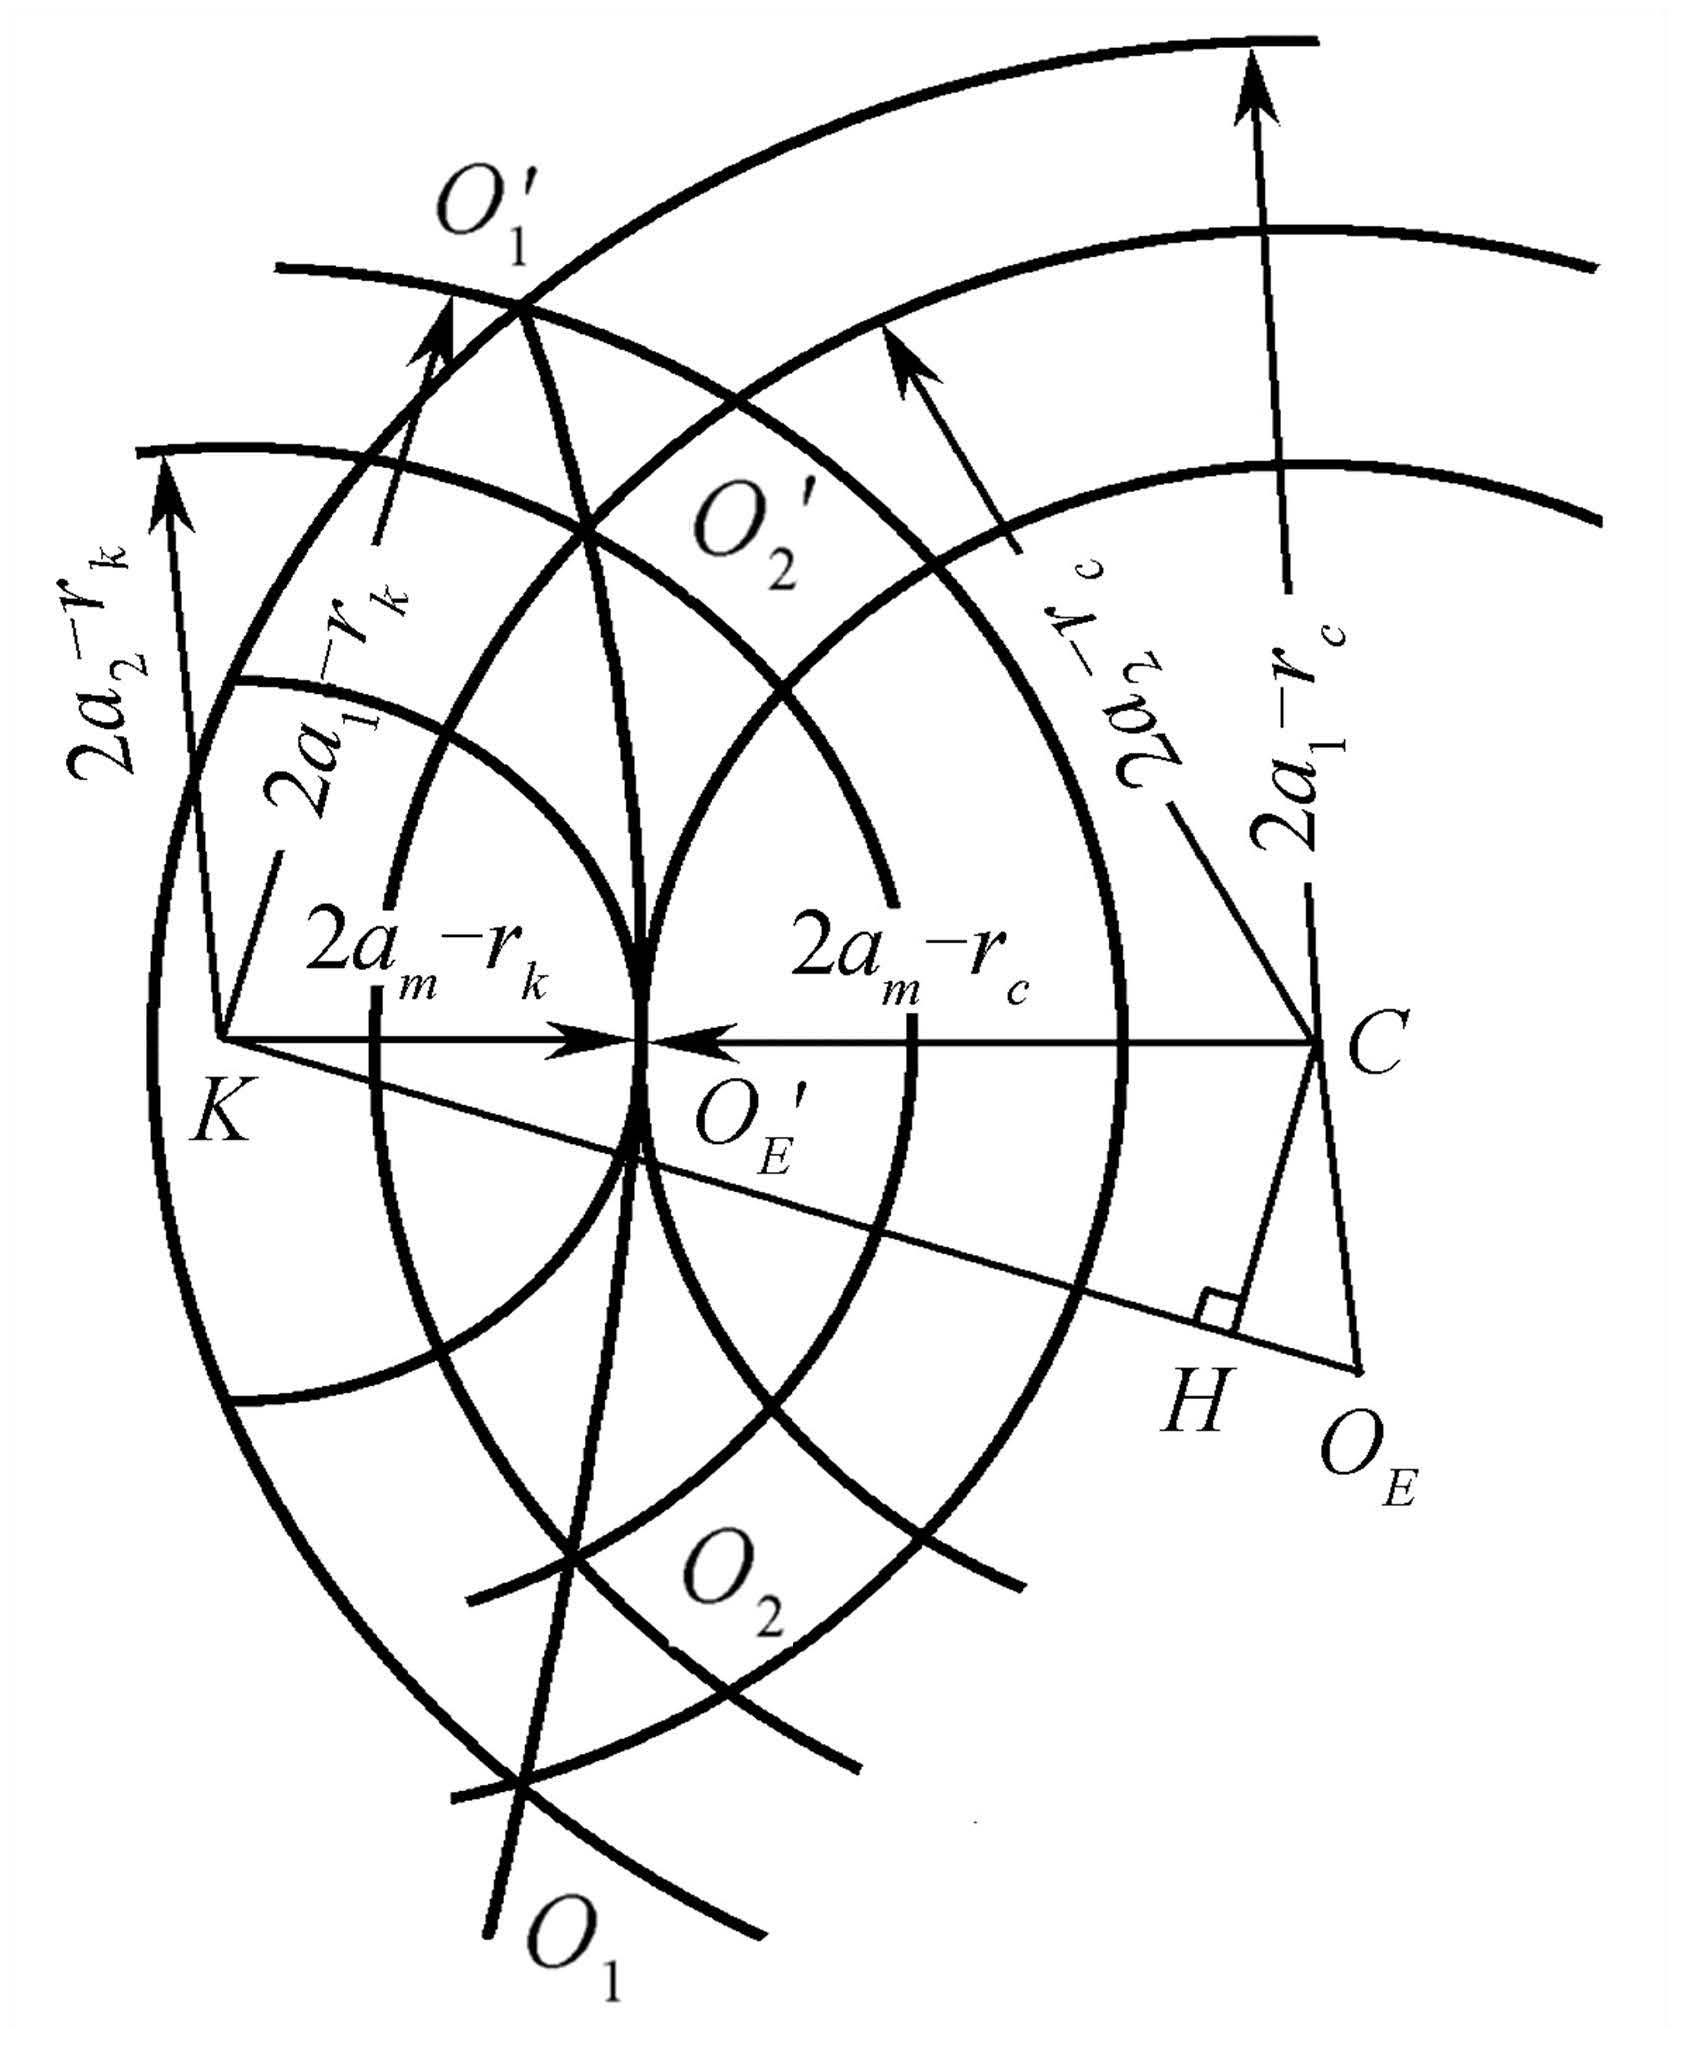
\includegraphics[width=0.3\linewidth]{pic/最小能量-最佳倾角.jpg}
	\vspace*{-1em}
	\caption{最小能量弹道图解法示意图}
	\label{最小能量}
\end{figure}

将再入段看成自由段的延续,被动段弹道为平面弹道。给定射程时,点$O_E, K, C$相对位置确定。设与地心$O_E$对应的椭圆虚焦点为$O$,满足
\begin{equation}
	\begin{cases}
		r_k + OK = 2a_k \\
		r_c + OC = 2a_c
	\end{cases} \qquad 
	\begin{cases}
		OK = 2a_k - r_k \\
		OC = 2a_c - r_c
	\end{cases}
\end{equation}

给定椭圆长半轴$a$,以$K,C$为圆心,分别以$OK$与$OC$为半径画圆,则有两个交点$O,O'$,即为椭圆虚焦点,对应椭圆的焦距、偏心率不同,如图\ref{最小能量}所示。可以得到

(1) \hspace*{0.5em} 两个虚焦点$O,O'$对称于$KC$连线。

(2) \hspace*{0.5em} 随着长半轴$a$减小,虚焦点逐渐靠近$KC$线,最终重合于$OE'$点。此时有
\begin{equation}
	a_{\min} = \dfrac{1}{4} \big(KC + r_k + r_c\big)
\end{equation}
长半轴最小,即能量最小,对应于最小能量弹道。















